\begin{figure}
\centering
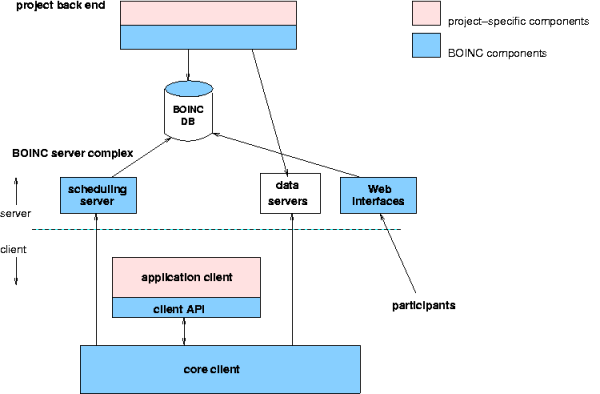
\includegraphics[scale=0.5]{figures/project_boinc}
\medskip
\caption{\textit{BOINC Client/Server Architecture} [5]}
\small
\end{figure}

\section{Rewarding Researchers}

Gridcoin does not only want to reward holders of the coin (as in pure Proof of Stake coins such as Peercoin [2]), but wants to reward researchers. Because of this there is an additional reward depending on the amount of research done. This information is read from a superblock. In some blocks, called superblocks, the majority consensus from the distributed Neural Network, which user has done how much work is also saved as a hash. These blocks are generated once a day. The current amount of research done by each CPID stored in the last superblock can be viewed on [SUPER]. If a node gets chosen and the hash this node contains about the amount of work done by each user is the same as the majority hash stored in the Neural Network, then this node gets to stake the next block and everything starts again. The actual reward the node gets then depends on the \textit{RAC} (Recent Averaged Credit [22]) for each project for this user as stored in the superblock.\\

\subsection{Cobblestone}

To understand \textit{RAC}, we first look at the \textit{cobblestone} [22]. The \textit{cobblestone} is a unit of measure defined as follows: it is 1/200 day (=7 minutes and 12 seconds, 432 seconds) of CPU time on a reference computer that does 1 Gigaflop (= 1 billion floating point operations per second) based on the Whetstone benchmark. A \textit{cobblestone} in other words correspond to 432 seconds * 1 Gigaflop = 432 billion floating point operations.\\


\subsection{Recent Averaged Credit (RAC)}

Recent Averaged Credit is calculated every time a user is granted new credit in form of cobblestones. Credits are exponentially averaged with a given half life of one week. Following explanation and figures are taken from [31]:\\

First, we define a decay function over seven days (t is given in days):\\

\begin{equation}
d(t) =  \mathrm{e}^{-t \cdot  ln(2) / 7}  
\end{equation}

As you can see in the graph below after one week the value is exactly halve, a week later it is again halved. Also note that after a half day the value has dropped to 0.95. It is a continuous mechanism. 7 is said to be the half life of the function. [31]\\


\begin{figure}
\centering
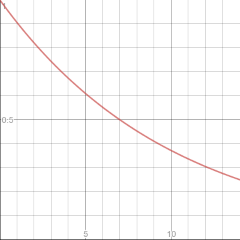
\includegraphics{figures/halflife}
\medskip
\caption{\textit{Decay function d(t) with a half life of 7 days }}
\small
\end{figure}


We now take an infinite impulse response low-pass filter with $\alpha$ as smoothing factor:

\begin{equation}
new\_value = \alpha \cdot old\_value + (1-\alpha) * new\_input
\end{equation}

The following graph gives an impression on how the above function behaves. As the input jumps to 1 the output slowly follows and wants to go to 1 as time passes. When the input changes this just repeats. This is called low pass because the output will only follow slow changes, at relevantly low frequencies. The input’s fast short jump to 2 didn’t really make it to the output. [31]\\

\begin{figure}
\centering
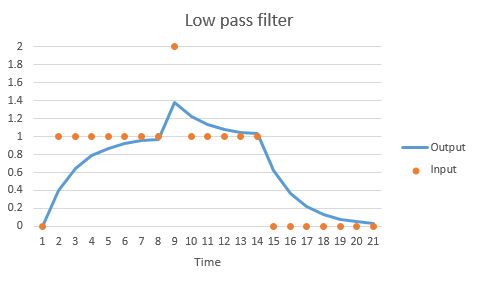
\includegraphics{figures/low-pass}
\caption{\textit{A low pass filter in action smooths spikes and dips}}
\small
\end{figure}


To get the formula for Recent Average Credit, we use the decay function $d(t)$ as smoothing facgtor in the infinite impulse response low pass filter:

\begin{equation}
RAC(new) = RAC(old) \cdot d(t) + (1-d(t)) \cdot credit(new)
\end{equation}

where $credit(new)$ is the credit in cobblestones for a calculated workunit issued in instant $t$.

\subsection{Gridcoin Payout to a user running multiple projects}

We hereby define:
\begin{description}
  \item{$\gamma$} : this is the average \textit{RAC} done by a user on a particular BOINC project \textit{p} since last payment to user \textit{u} identified by \textit{CPID}.
  \item{$\Gamma$} : this is the average \textit{RAC} done by all users participating in Gridcoin on a particular BOINC project \textit{p} since last payment to user \textit{u}.
  \item{$\tau$} : this is the time expressed in days since last payment to user \textit{u}.
  \item{$\Theta$} : this is the available Gridcoin supply per day assigned to BOINC project \textit{p}
  \item{$G$} : this is the constant number of Gridcoins created per day on the Gridcoin network. 
  \item{$n$} : this is the number of BOINC projects in the whitelist [42]. Participants in whitelisted projects do receive a reward in Gridcoins for their computational effort.  
\end{description}

The ratio
\[\gamma/\Gamma\]
is the percentage of work done by user \textit{u} on BOINC project \textit{p} in respect to all other Gridcoin users working on project \textit{p}.\\

The amount of coins $\sigma$ for project \textit{p} the user \textit{u} gets, if he was only running project \textit{p}, is computed:
\[ \sigma = (\gamma / \Gamma) \cdot \tau \cdot \Theta \]

As of now the $\Theta$ is the same for each project, so
\[ \Theta = G/n \]

$\gamma$ and $\Gamma$ are calculated so that in case there were several superblocks since the last payment the average RAC of all those superblocks is used.\\

The $researchreward$ for user \textit{u} is then the sum of the rewards for each whitelisted project:

\[ researchreward = \sum_{p=1}^{n} \sigma(p) \]


The $totalreward$  for user \textit{u} is then the reward for the research done by this node plus the reward that any node gets for staking a block, called $inflationreward$ in the next formula:
\[ totalreward = inflationreward +  researchreward \]

The $inflationreward$ depends on the time that passed since the last stake is chosen in a way that it leads to an interest rate of 1.5\% per year.\\

The rewards that contain only $inflationreward$ and no $researchreward$
are often called PoS (Proof of Stake) rewards, whereas the rewards containing $inflationreward$ plus $researchreward$ are called Proof of Research rewards.
